\documentclass[12pt,fleqn]{article}\usepackage{../../common}
\begin{document}
Testlere Devam 

İstatistiki test yaratmak için takip edilen teknik basit; bir istatistiki
ölçüt hesaplıyoruz, ya da hesabımızın başka noktasından çıkanı alıyoruz, ki
bu ölçüt mesela bir ortalama olabilir bu durumda bilinen bir dağılımı
vardır, ya da lineer regresyondan bize verilen bir katsayıdır, onun t
değeri vardır, bu durumda da dağılımın ne olduğunu biliyoruz. Yani hangi
ölçüte bakarsak bakalım, ya da biz yeni bir tanesini uyduralım, önce elde
ettiğimiz rasgele değişkeninin ideal koşullarda dağılımının ne olduğuna
bakarız, ki test ettiğimiz bir anlamda bu ideal koşullar
olacaktır. Ardından bir kriter ortaya koyarak testi ortaya çıkartırız.

Ama ondan önce biraz regresyon.

Örnek veri olarak Big Andy's Burger Barn adında hamburger satan bir
restoran zincirinin verisini kullanalım [1, sf. 168]. Veride her nokta ayrı
bir şehirdeki belli bir aydaki dükkan için kaydedilmiş reklam gideri
$ADVERT$, burger fiyatı $PRICE$, ve satış getirisi $SALES$ ($SALES$ ve
$ADVERT$ bin dolarlık birimde kaydedilmiş). Şirket yönetimi diyelim ki
reklam harcamalarının satışları nasıl etkilediğini merak ediyor. Ayrıca
yönetim bir fiyatlama stratejisi belirlemek istiyor, fiyatın geliri nasıl
etkilmektedir? Fiyatta düşüş çok az satış artışı yaratıyorsa bu durum
kazancı düşürür, demek ki talep fiyatsal-elastik değildir (price
inelastic). Tam tersi de olabilir, fiyat değişimi satışı arttırır, o zaman
talep fiyatsal-elastiktir.

\begin{minted}[fontsize=\footnotesize]{python}
import pandas as pd
df = pd.read_csv('andy.dat',sep='\s*',names=['sales','price','advert'])
print df.head(3)
\end{minted}

\begin{verbatim}
   sales  price  advert
0   73.2   5.69     1.3
1   71.8   6.49     2.9
2   62.4   5.63     0.8
\end{verbatim}

Regresyon modelini kuralım,

$$ SALES = \beta_1 + \beta_2 PRICE + \beta_3 ADVERT $$

\begin{minted}[fontsize=\footnotesize]{python}
import statsmodels.formula.api as smf
results = smf.ols('sales ~ price + advert', data=df).fit()
print results.summary()
\end{minted}

\begin{verbatim}
                            OLS Regression Results                            
==============================================================================
Dep. Variable:                  sales   R-squared:                       0.448
Model:                            OLS   Adj. R-squared:                  0.433
Method:                 Least Squares   F-statistic:                     29.25
Date:                Mon, 24 Aug 2015   Prob (F-statistic):           5.04e-10
Time:                        08:59:52   Log-Likelihood:                -223.87
No. Observations:                  75   AIC:                             453.7
Df Residuals:                      72   BIC:                             460.7
Df Model:                           2                                         
Covariance Type:            nonrobust                                         
==============================================================================
                 coef    std err          t      P>|t|      [95.0% Conf. Int.]
------------------------------------------------------------------------------
Intercept    118.9136      6.352     18.722      0.000       106.252   131.575
price         -7.9079      1.096     -7.215      0.000       -10.093    -5.723
advert         1.8626      0.683      2.726      0.008         0.501     3.225
==============================================================================
Omnibus:                        0.535   Durbin-Watson:                   2.183
Prob(Omnibus):                  0.765   Jarque-Bera (JB):                0.159
Skew:                          -0.072   Prob(JB):                        0.924
Kurtosis:                       3.174   Cond. No.                         69.5
==============================================================================
\end{verbatim}

Fiyatsal elastikliği kontrol etmek için $\beta_2$'nin t değerine
bakabiliriz çünkü bu değer $\beta_2=0$ hipotezini reddedip
reddedemeyeceğimiz hakkında bize bir şeyler söylüyor. Eğer t değer ve
\verb!P>|t|! değeri 0.05'ten küçük ise hipotezi reddedebiliriz. Çıktıya
bakıyoruz, 0 değerini görüyoruz. Demek ki fiyatsal elastiklik vardır. 

Gayrı Lineerlik: Fakat acaba reklam harcaması ile satış arasında tam lineer
bir ilişki mi var? Belli bir noktadan sonra ne kadar harcarsak harcayalım
daha fazla kazanamayacağımız bir durum da olamaz mı? Bunu test edelim,
$ADVERT^2$ değişkenini ekleyip yeni bir regresyon yaratalım. $ADVERT$'in
karesini aldık çünkü karesi alınmış $ADVERT$ normal olana göre daha hızlı
büyür, yani büyük değerlerde karesinin sonucu çok daha büyüktür, ve eğer bu
uç noktalarda bir kalıp var ise, onu ``yakalamak'' bu karesi alınmış yeni
değişken sayesinde mümkün olur.

\begin{minted}[fontsize=\footnotesize]{python}
import statsmodels.formula.api as smf
df['advert2'] = df.advert**2 # kare aldik
results2 = smf.ols('sales ~ price + advert + advert2', data=df).fit()
print results2.summary()
\end{minted}

\begin{verbatim}
                            OLS Regression Results                            
==============================================================================
Dep. Variable:                  sales   R-squared:                       0.508
Model:                            OLS   Adj. R-squared:                  0.487
Method:                 Least Squares   F-statistic:                     24.46
Date:                Mon, 24 Aug 2015   Prob (F-statistic):           5.60e-11
Time:                        15:54:13   Log-Likelihood:                -219.55
No. Observations:                  75   AIC:                             447.1
Df Residuals:                      71   BIC:                             456.4
Df Model:                           3                                         
Covariance Type:            nonrobust                                         
==============================================================================
                 coef    std err          t      P>|t|      [95.0% Conf. Int.]
------------------------------------------------------------------------------
Intercept    109.7190      6.799     16.137      0.000        96.162   123.276
price         -7.6400      1.046     -7.304      0.000        -9.726    -5.554
advert        12.1512      3.556      3.417      0.001         5.060    19.242
advert2       -2.7680      0.941     -2.943      0.004        -4.644    -0.892
==============================================================================
Omnibus:                        1.004   Durbin-Watson:                   2.043
Prob(Omnibus):                  0.605   Jarque-Bera (JB):                0.455
Skew:                          -0.088   Prob(JB):                        0.797
Kurtosis:                       3.339   Cond. No.                         101.
==============================================================================

\end{verbatim}

Yeni regresyon için $R^2=0.50$! Bu yeni model verideki varyansın yüzde
50'sini açıklıyor! Eskisinden daha iyi bir model ve AIC'i de daha düşük
zaten, ve $ADVERT^2$ için hesaplanan katsayı -2.768 eksi değeri
taşıyor. Demek ki reklam harcamalarının belli bir noktadan sonra etkisinin
aynı olmayacağı varsayımımız doğru. 

Birleşik Hipotez Testleri

Ne yazık ki t testi ile ortak (joint) hipotez testleri
yapamıyoruz. Mesela sadece bir değil, {\em birkaç değişkenin} model için ne
kadar önemli olduğunu bilmek istiyoruz. Tabii bu değişkenleri regresyondan
atabiliriz, sonra çıplak gözle AIC'e bakarız, vs. Fakat bu testi daha
İstatistiksel bir hipotez testi olarak yapmak daha iyi olmaz mıydı? Alttaki
test bu durumlar için kullanılır,

F Testi

Diyelim ki reklam harcamasının satışı etkileyip etkilemediğini merak
ediyoruz. Fakat artık bir değil iki tane reklam ile alakalı değişkenimiz
var! Biri $ADVERT$ diğeri onun karesi $ADVERT^2$. Sıfır hipotezimiz şu
olacak, ``reklam harcaması satışları belirlemede etkili değildir''. Yani 

$$ H_0: \beta_3=0, \beta_4=0 $$

$$ H_1: \beta_3 \ne 0, \textrm{ ya da } \beta_4 \ne 0 \textrm{ ya da ikisi
  de sıfır değil} $$

Hipotez bu şekilde tanımlanınca onu reddetmek demek reklamın satışları
etkilediği hakkında güçlü bir kanıt ortaya koyar. Bu nokta önemli, aşırı
fantastik bir şekilde zaten umduğumuz şeyi desteklemek için kanıt aramak
yerine, onun tam tersini reddetmek için kanıt arıyoruz. 

Peki bu testi nasıl yaratacağız? Bir regresyona değişken eklemek onun
hatasını azaltır, çıkartmak ise çoğaltır. Eğer ana regresyondan değişken
çıkartırsak onun hatası $SSE_u$ diyelim, çoğalarak $SSE_r$ olur. Notasyonel
açıdan değişik bir şekilde de duruma bakabiliriz, $\beta_3=0, \beta_4=0$
şartını koşmak aslında bir modeli kısıtlamak ta (restrict) anlamına gelir,
üzerinde şart belirlenmemiş olan model de kısıtlanmamış (unrestricted)
olur. Neyse, F testi ile yapmaya çalışacağımız bu çoğalmanın istatistiki
olarak önemli (significant) olup olmadığını anlamaktır. $SSE$ notasyonu bu
arada hata karelerinin toplamı (sum of squared errors) kelimelerinden
geliyor.

Şimdi, daha önce belirttiğimiz gibi, ideal şartlarda doğru olacak bir ölçüt
yaratmak, ve bu ideal şartlarda bu ölçütün dağılımını bulmak, ve veriyi
kullanıp bu ölçütü hesaplayıp sonucu bu dağılıma ``sormak''
gerekiyor. Eğer sıfır hipotezi doğru ise,

$$ F = \frac{(SSE_r - SSE_u)/j}{SSE_u/(n-k)} $$

hesabı bir $F_{j,n-k}$ dağılımıdır. F dağılımının tanımını hatırlayalım,
iki chi kare dağılımının birbiriyle bölünmüş hali idi,

$$ F_{j,n-k} = \frac{\chi^2 / j}{\chi^2 / n-k} $$

SSE hesapları karelerin toplamı olduğu için ve hataların normal dağıldığı
varsayımından hareketle bölüm ve bölendeki rasgele değişkenler Chi kare
dağılımına sahiptir.

Peki neden üstteki F dağılımının $j,n-k$ derece serbestliği vardır? İki chi
kare dağılımını toplayınca onların dereceleri toplanır. Aynı şekilde
çıkartma derece eksiltir. Şimdi, $SSE_r$'nin derecesi $n-k$'dir, $k$ tane
katsayı dereceyi / serbestliği azaltmıştır. Eğer $SSE_r$ elde etmek için
$j$ tane katsayıyı çıkartırsak, bu durum dereceyi fazlalaştırır, yani
$SSE_r$ için $n-k+j$ elde ederiz. O zaman bölümdeki çıkartmanın derecesi

$$ (n-r+j) - (n-r) = j$$

olacaktır. Şimdi nihai hesabı yapalım, regresyonu reklamla alakalı iki
değişkeni çıkartılmış şekilde bir daha işletiriz, sonra SSE hesabı için her
iki regresyondan gelen artıklar \verb!resid!'leri kullanırız, onların
karelerinin toplamı bize gerekli $SSE$ hesabını verecektir,

\begin{minted}[fontsize=\footnotesize]{python}
import statsmodels.formula.api as smf
results3 = smf.ols('sales ~ price ', data=df).fit()
SSE_u = np.sum(results2.resid**2)
SSE_r = np.sum(results3.resid**2)
print 'SSE_u', SSE_u
print 'SSE_r', SSE_r
J = 2; N=len(df); K = len(results2.params)
F = (SSE_r - SSE_u)/J / SSE_u*(N-K)
print 'j,n-k',J,N-K
print 'F =', F
\end{minted}

\begin{verbatim}
SSE_u 1532.0844587
SSE_r 1896.39083709
j,n-k 2 71
F = 8.44135997807
\end{verbatim}

p değeri $P(F_{j,n-k}>8.44)$. Kumulatif yoğunluk fonksiyonu (CDF)
kullanabilmek için formülü şu şekilde tekrar yazalım,
$1-P(F_{j,n-k}<8.44)$,

\begin{minted}[fontsize=\footnotesize]{python}
import scipy.stats as st
f = st.f(J,N-K)
print 1-f.cdf(F)
\end{minted}

\begin{verbatim}
0.000514159058424
\end{verbatim}

Üstteki değer 0.05 kritik değerinden daha ufak olduğu için hipotez
reddedilmiştir. Direk p değeri hesabı yerine yüzde 95 güven için bir eşik
değeri de hesaplayabilirdik,

\begin{minted}[fontsize=\footnotesize]{python}
print f.ppf(0.95)
\end{minted}

\begin{verbatim}
3.12576423681
\end{verbatim}

Ve eğer F değeri bu değerden büyük ise hipotez reddedilmiştir diyebilirdik,
ki hesapladığımız F değeri eşik değerinden büyük idi. Vardığımız sonuç
reklam harcamalarının satış için önemli olduğudur.

Daha Basit bir F-Test Örneği

F-Test'in ana fonksiyonu ve ilk kullanımı varyans karşılaştırmak aslında,
iki ölçüm grubunu standard sapma karesinin oranı alınır, ve sonuç bir F
rasgele değişkenidir, belli serbestlik dereceleri vardır,

$$ F = \frac{S_x^2}{S_y^2} $$

ki $S_x,S_y$ 1. ve 2. grubun örneklem standart sapmasıdır. Bu şekilde bir
örnek te görelim [2, sf. 42]. Diyelim ki elimizde göz hareketlerini ölçen
iki metod var, gözümüzü 20 derece hareket ettirince metotlar şu rakamları
veriyor,

\begin{minted}[fontsize=\footnotesize]{python}
method_1 = [20.7, 20.3,20.3, 20.3, 20.7, 19.9, 19.9, 19.9, \
            20.3, 20.3, 19.7, 20.3]
method_2 = [19.7, 19.4, 20.1, 18.6, 18.8, 20.2, 18.7, 19.]
\end{minted}

F-testini kullanarak bu metotların, ölçümlerin doğruluğunun (accuracy) aynı
mı, yoksa birinin diğerinden daha doğru mu olduğunu bulacağız. 

\begin{minted}[fontsize=\footnotesize]{python}
import pandas as pd
m1 = np.array(method_1); m2 = np.array(method_2)
df = pd.DataFrame([m1,m2]).T
ss = df.std()
F = ss.ix[0]**2/ss.ix[1]**2
print F
\end{minted}

\begin{verbatim}
0.243934673841
\end{verbatim}

\begin{minted}[fontsize=\footnotesize]{python}
import scipy.stats as st
f = st.f(len(m1)-1,len(m2)-1)
print 1-f.cdf(F)
\end{minted}

\begin{verbatim}
0.981334830069
\end{verbatim}

F dağılımı $n-1 ve $m-1$ serbestlik derecesine sahip. $ Üstteki p değeri
0.05'ten küçük değildir, demek ki iki metotun ölçüm doğruluğunun aynı olduğu
hipotezini reddedemiyoruz. Not: Örneklem standart sapma hesabı için $n-1$'e
bölünme durumu var, bu bölüm kullanılan $F$'in derecesine yansıyor tabii.

Testin özünde şu var, ki varyansın eşitsizliği oranın 1'den ne kadar uzak
olduğuna bağlı. Ama ne kadar uzak istatistiki olarak önemli bir uzaklık? İşte
bunun cevabını F-dağılımı veriyor. 

Örneklem Korelasyonu 

Korelasyon $\rho$'yu daha önce gördük, tahmin edicisi $r$'dir, 

$$ 
\hat{\rho} = r = \frac{S_{xy}}{\sqrt{S_{xx}S_{yy}}} 
\mlabel{1} 
$$

ki örneklem hesapları $S_{xx},S_{xy},S_{yy}$ 

$$ S_{xx} = \sum _{i=1}^{n} (x_i-\bar{x})^2 $$

$$ S_{xy} = \sum _{i=1}^{n} (x_i-\bar{x})(y_i-\bar{y}) $$

$$ S_{yy} = \sum _{i=1}^{n} (y_i-\bar{y})^2 $$

olsun; bu hesapların teorik varyans ile olan bağlantısı görülebilir. Eğer
$X,Y$ iki değişkenli (bivariate) bir normal dağılımından geliyorsa, o zaman
ortada bir regresyon varmış gibi gösterebiliriz

$$ E(Y|X=x) = \beta_0 + \beta_1 x + \epsilon $$

ki $\beta_1 = \sigma_Y / \sigma_X \cdot \rho$ olur. Detaylar için [4]. Soru şu, $r$ için bir  istatistiksel 
önemlilik (significance) hesabı nasıl yapardık? Yani, eğer $-1 \le r \le 1$
işe,  ve $r=0$ hiç korelasyon olmama durumu ise, acaba bu ``sıfır olmama'' 
durumunu test edebilir miydim? Evet. Yukarıdaki normallik faraziyesi doğru 
ise $\beta_1 = 0$ olmama durumunu test etmek $\rho = 0$ olmama testi ile aynı, bu durumda

$$ t_0 = \frac{\hat{\beta_1}}{\sqrt{ Var(\hat{\beta_1} ) }} $$

gibi bir test istatistiği yaratırız, ki bu istatistik Öğrenci t dağılımına
sahip olurdu çünkü sıfır hipotezi $\hat{\beta_1} = 0$, ve üstteki
istatistik sıfır hipotezi altında ile Öğrenci t dağılımına sahip olmak
zorundadır, çünkü bölünen normal dağılmış, bölen chi karenin karekökü
olarak dağılmış. Eğer $t_o$ hesabı veriye uygulandıktan sonra hipotezin
öngördüğü dağılıma uymaz ise, sıfır hipotezini reddederiz. 

Bu noktada lineer regresyon ile alakalı bilgiler devreye sokulabilir,
[4]'den biliyoruz ki

$$ Var(\hat{\beta_1}) = \frac{\sigma^2}{S_{xx}} $$

$\sigma$ yerine örneklemden gelen $S$ kullanırsak ve üstteki formüle koyarsak,

$$ t_0 = \frac{\hat{\beta_1}}{\sqrt{S / S_{xx}}} $$

Bu ifadeyi $r$ bazında ifade edebilir miyiz?  Deneyelim, $\hat{\beta_1} =
S_{xy} / S_{xx}$ ve $r = \hat{\beta_1}\sqrt{\frac{S_{xx}}{S_{yy}}}$ olduğunu
biliyoruz [4], ayrıca

$$ S = \frac{SSE}{n-2}, \qquad SSE = S_{yy} - \hat{\beta_1} S_{xy} $$

ki $SSE$ hata karelerinin toplamıdır (sum of squared errors),

$$ t_0 = \frac{  \sqrt{S_{xx}} \hat{\beta_1} \sqrt{n-2} }{\sqrt{SSE}} $$

$$ = \frac{  \sqrt{S_{xx}} \hat{\beta_1} \sqrt{n-2} }{\sqrt{S_{yy} - \hat{\beta_1} S_{xy}}} $$

Bölümün iki kısmını $\sqrt{S_y}$ ile bölelim, 

$$ = 
\frac{ \sqrt{S_{xx}/S_{yy}} \hat{\beta_1} \sqrt{n-2} }
{\sqrt{1 - \hat{\beta_1} S_{xy}/S_{yy}}} 
$$

Bölünen kısmında bir $r$ ortaya çıktı,

$$ = 
\frac{ r\sqrt{n-2} }
{\sqrt{1 - \hat{\beta_1} S_{xy}/S_{yy}}} 
$$

Bölen kısmındaki $\hat{\beta_1}$ yerine $\hat{\beta_1} = S_{xy} / S_{xx}$
koyarsak yine (1)'deki $r$ tanımına geliriz, ve alttaki basitleştirilmiş
ifade ortaya çıkar,

$$ t_o = \sqrt{\frac{(n-2)r^2}{(1-r^2)}} $$

Bu istatistik $n-2$ derece serbestliğe sahip bir Öğrenci t dağılımıdır. 

Örnek

Possum adı verilen bir tür hayvanın dişilerinin tüm uzunluğu ve kafa ölçümü
\verb!totlngth,hdlngth! değişkenleri arasında korelasyon olup olmadığı
merak edilmektedir.

\begin{minted}[fontsize=\footnotesize]{python}
import pandas as pd
import scipy.stats

def p_corr(df1, df2):
    corr = df1.corr(df2)
    N = np.sum(df1.notnull())
    t = corr*np.sqrt((N-2)/(1-corr**2))
    p = 1-scipy.stats.t.cdf(abs(t),N-2)  # one-tailed
    return corr, t, p

df = pd.read_csv('fossum.csv')
c,tval, pval = p_corr(df.totlngth,df.hdlngth)
print c, pval
\end{minted}

\begin{verbatim}
0.779239322172 3.75045772216e-10
\end{verbatim}

p-değeri çok küçük, demek ki korelason olmadığı tezi reddedildi. Korelasyon
var.

Pearson Chi Kare Uyum Derecesi (Goodness-of-Fit) Testi

Her sene günde kaç saat çalıştığımızı bir yere yazdık diyelim, elde 365
veri noktası var. Ertesi sene yine aynı veriyi topladık, şu soruyu
soruyoruz, iki veri birbirinden istatistiki olarak farklı mıdır?  Ya da;
elimizdeki belli bir veri var, ve o verinin normal mi, ya da üstel
(exponential) dağılımdan mı geldiğini merak ediyoruz. Acaba veri
istatistiki olarak hangi {\em tip} dağılım fonksiyona (yani teorik yoğunluk
fonksiyonuna) daha yakındır? Ya da; eldeki bir verinin $\mu = 0$ merkezli
normal dağılımdan mı, yoksa $\mu = 30$ merkezli normal dağılımdan mı
geldiğini merak ediyoruz.

Her üç sorunun ve benzerlerinin cevabı Pearson'un chi kare (chi square)
uyum derece testi ile verilebilir. 

İki veriyi karşılaştırdığımız durumda bu iki veri kümesini dağılım olarak
kabul edip, birini diğerine uyum açısından test edebiliriz. Bu
karşılaştırma her iki tarafta histogram alınıp histogram kutucuklarının
(bins) içine her iki tarafta düşen miktarların bir test istatistiği
üzerinden karşılaştırılması ile olabilir. Veri ile yoğunluk
karşılaştırdığımızda ise veriyi histogram kutucukları, yoğunluğu ise aynı
aralıklara düşen olasılıkların fonksiyonel hesaplarıyla karşılaştırılması
ile yaparız. 

Test istatistiği 

Diyelim ki her kutucukta görülen miktar $N_i$, ki $N_1 + N_2 + .. + N_k =
n$, ve karşılaştırmak istediğimiz, bu miktara tekabül eden ``ideal''
olasılık $p_i$, o zaman ideal miktar $n p_i$. Kutucuktaki sayıları bir
binom dağılımından geliyormuş gibi modelleyebiliriz, 1. kutucuk için mesela
$N_1 \sim Bin(n,p_1)$, ve $N_1$ rasgele değişkeni $N$ tane deneyde
``başarılı'' olan sayı - tipik binom kullanımı. Bu durumda Pearson uyum
derecesi istatistiği

$$
\chi^2 = \sum_{j=1}^{k} \frac{(N_j - np_j)^2}{np_j}
$$

ile belirtilir, üstteki toplamın yaklaşıksal olarak $\chi^2_{k-1}$
dağılımına yaklaştığı ispatlanmıştır. Detaylar için [5, sf 318, 6]. Nihai
ispat oldukça çetrefil, biz burada alternatif bazı yaklaşıksal ispatlardan
bahsetmek istiyoruz (okkalı ispat için yukarıdaki referanslar geçerli
tabii).

Eğer her $N_j$ binom dağılımını Gaussian ile yaklaşıkladığımızı düşünürsek,
ki bu yeterince büyük $n$, ve $np_i>5$ için mümkün, bu dağılım $\mu=np_j$
ve varyans $np_j(1-p_j)$'ye sahip olur, o zaman Gaussian'ı standardize
etmek için

$$ \frac{N_j-np_j}{\sqrt{np_j(1-p_j)}} \approx N(0,1) $$

$Z=N(0,1)$ diyelim,

$$
\frac{(N_j - np_j)}{\sqrt{np_j} } \approx  \sqrt{(1-p_j)}Z
$$

İki tarafın karesini alalım, ve her $j$ üzerinden toplam alalım,

$$
\sum_j \frac{(N_j - np_j)^2}{np_j} \approx \sum_j (1-p_j)Z^2
$$

Üstteki eşitliğin sol tarafı Pearson istatistiğiyle aynı. Sağ tarafı neye
eşit? 

$$
\sum_j (1-p_j)Z^2 =  (1-p_1)Z^2 + (1-p_2)Z^2 + ... + (1-p_k)Z^2 
$$

$$
 =  Z^2 [(1-p_1) + (1-p_2) + ... + (1-p_k)]
$$

$$
 =  Z^2 [k - (p_1+p_2+..+p_k))] = (k-1)Z^2 = \sum_{k-1} Z^2 
$$

Şimdi, bu eriştiğimiz toplamın $\chi^2_{k-1}$ dağılımı, yani $k-1$ derece
serbestliği olan bir chi kare dağılımı olduğunu iddia edebilir miyiz? Eğer
$Z_j$'ler birbirinden bağımsız ise kesinlikle evet, çünkü standart normal
rasgele değişkenlerin toplamı chi kare dağılımını verir. Üstteki kolay
ispatın önündeki tek engel budur, bizim burada yapacağımız yaklaşıksal
argüman $i,j$ ikilisi için $Z$'lerin bağlantısının, kovaryansının küçük
olduğudur, ki bu küçüklük sebebiyle $Z_j$'ler çoğu durumda bağımsız kabul
edilebilir.

Diyelim ki $X_1,X_2,..$ değişkenleri bağımsız ve $Mult(1,p)$, yani multinom 
dağılımdan geliyorlar [7, sf. 180], ve $p = \left[\begin{array}{ccc} p_1 & p_2 &
 \dots \end{array}\right]$, ve $\sum_j p_j = 1$. 
Yani her $X_i$ zar attığında $1 \times k$ boyutlu bir vektör ortaya çıkıyor, bu vektörün
sadece bir hücresi 1 diğerleri 0. Multinom dağılımların
tanımından biliyoruz ki $Cov(X_i,X_j) = -n p_ip_j = -p_ip_j$ (çünkü $n=1$). 

Bu demektir ki 1'den küçük iki değer çarpılıyor bu daha da küçük bir değer
verecektir. Eğer $k$ yeterince büyük ise, bu, mesela sürekli yoğunlukları
ayrıksal olarak gösterdiğimiz durumda ve yeterince çok kutucuk var ise bu
kutucuklara ``düşen'' olasılıkların ufalması demektir, ve ufak değerlerin
çarpımı iyice ufalır, ki bu kovaryansı sıfıra yaklaştırır. Yani yeterince
büyük $k$ için $i,j$ bağlantısını sezgisel bağlamda etkisiz olduğunu
görebiliriz. Tabii, toplamın {\em kesinlikle} chi kare olduğunun ispatı
için dediğimiz gibi verdiğimiz referanslara bakılabilir. 

İstatistiki testlerin mantığını hatırlarsak, tarif edilen Pearson
istatistiği sıfır hipotezi. Bize reddetmeye uğraşacağımız bir dağılım /
hesap ikilisi üretiyor. Eğer hesap beklenen, normal (sıfır hipotez durumu)
uymuyorsa, hipotezi reddediyoruz. Ret durumu özellikle seçiliyor çünkü
kabul edilmezlik daha kesin bir cevap. 

Örnek

Bir paralı otoyolunda geçiş noktasında durulmuş ve her dakika gelen araç
sayılmış, ve dakika başına bu araç sayısı yazılmış. Bu deney 106 dakika
süresince yapılmış (elde 106 satırlı bir veri var yani). Bu veri için
Poisson dağılımının uygun olup olmadığını yüzde 5 önemlilik seviyesinde
ispatlamamız isteniyor.

\begin{minted}[fontsize=\footnotesize]{python}
import pandas as pd
df = pd.read_csv('vehicles.csv',header=None)
\end{minted}

Verinin histogramına bakalım,

\begin{minted}[fontsize=\footnotesize]{python}
f = plt.figure(); df.hist(bins=13)
plt.savefig('stat_tests2_01.png')
\end{minted}

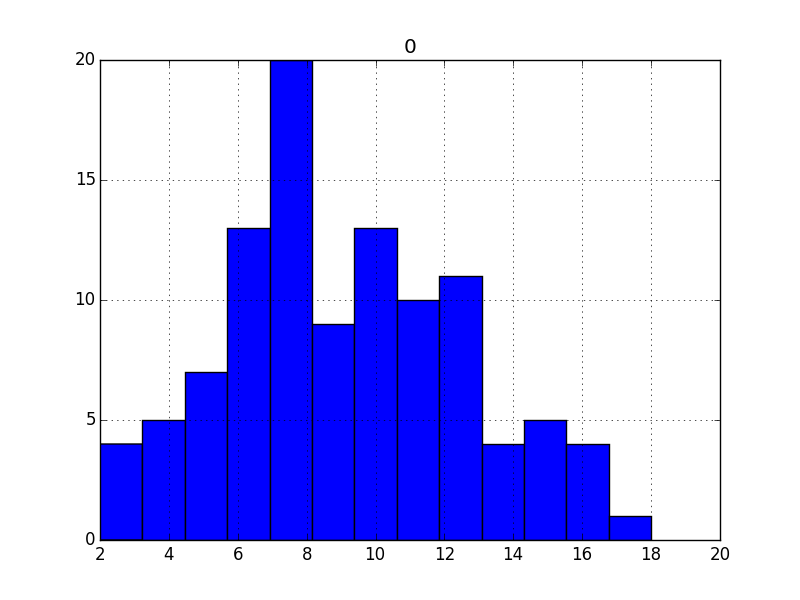
\includegraphics[height=6cm]{stat_tests2_01.png}

Poisson dağılımı muhtemel gözüküyor. Ama şimdi bunu uyum derece testi ile
daha kararlı şekilde göstermeye uğraşacağız. Verideki sayımları o sayım
rakamı bazında gruplayalıp gösterelim,

\begin{minted}[fontsize=\footnotesize]{python}
kt = plt.hist(np.array(df),bins=range(20))
kt = pd.DataFrame([kt[1],kt[0]]).T
kt = kt[:-1] # sonuncu satiri at
kt.columns = ['kac araba','kac kere']
print kt
\end{minted}

\begin{verbatim}
    kac araba  kac kere
0           0         0
1           1         0
2           2         1
3           3         3
4           4         5
5           5         7
6           6        13
7           7        12
8           8         8
9           9         9
10         10        13
11         11        10
12         12         5
13         13         6
14         14         4
15         15         5
16         16         4
17         17         0
18         18         1
\end{verbatim}

Yani bir dakikada 6 araba sayımı 13 kere yapılmış (13 değişik dakikada).

Bazı kutucukların boş olduğunu görüyoruz, bu durum özellikle tek tepeli
(unimodel) dağılımlı verilerde etekleri temsil eden uçlardaki kutucukların
boş olması sonucunu verebilir. Bu durumda o kutucukların verisi daha dolu
olanlara aktarabilmek için kutucuk noktalarını tekrar tanımlıyoruz,

\begin{minted}[fontsize=\footnotesize]{python}
bins = [0] + range(5,15) + [100]
kt2 = plt.hist(np.array(df),bins=bins)
kt2 = pd.DataFrame([kt2[1],kt2[0]]).T
kt2.columns = ['int_low','n_i']
print kt2
\end{minted}

\begin{verbatim}
    int_low  n_i
0         0    9
1         5    7
2         6   13
3         7   12
4         8    8
5         9    9
6        10   13
7        11   10
8        12    5
9        13    6
10       14   14
11      100  NaN
\end{verbatim}

Şimdi bu değerler üzerinden Pearson $\chi^2$ hesabını yapalım. Ama ondan
önce, hatırlayalım, bu verinin {\em herhangi bir} Poisson'dan gelip
gelmediğini kontrol ediyoruz, ama testimiz için parametresi belli olan,
özel bir Poisson lazım, bunun için bize bir $\lambda$ gerekiyor. Önemli
değil, $\lambda$'nin tahmin edicisi $\hat{\lambda}$'yi biliyoruz,

$$ \hat{\lambda} = \frac{1}{n} \sum _{j=1}^{n}x_j $$

Bu $\hat{\lambda}$'yi kullanarak Poisson hesaplarını yapabiliriz artık. Bir
kutucuğa düşen Poisson olasılığının hesabı $P(a \le X < b)$, ki bu basit
bir $F(b)-F(a)$, yani $a,b$ noktalarındaki kümülatif yoğunluk fonksiyonun
farkı üzerinden hesaplanabilir, altta kullanılan çağrı \verb!poisson.cdf!.

\begin{minted}[fontsize=\footnotesize]{python}
from scipy.stats import poisson
kt2['int_high'] = kt2.shift(-1).int_low
lam = df.mean() # tahmin edici
def f(x): 
   high = poisson.cdf(x.int_high-1,lam)
   low = poisson.cdf(x.int_low-1,lam)
   return pd.Series(high-low)
kt2['p_i'] = kt2.apply(f,axis=1)
kt2['np_i'] = len(df) * kt2['p_i']
kt2['chi'] = (kt2['n_i']-kt2['np_i'])**2 / kt2['np_i']
kt2 = kt2[:-1]
print kt2
print '\nchi kare istatistigi', kt2.chi.sum()
\end{minted}

\begin{verbatim}
    int_low  n_i  int_high       p_i       np_i       chi
0         0    9         5  0.051863   5.497487  2.231492
1         5    7         6  0.058217   6.171048  0.111352
2         6   13         7  0.088242   9.353602  1.421508
3         7   12         8  0.114643  12.152118  0.001904
4         8    8         9  0.130325  13.814437  2.447271
5         9    9        10  0.131691  13.959242  1.761849
6        10   13        11  0.119764  12.695009  0.007327
7        11   10        12  0.099016  10.495702  0.023412
8        12    5        13  0.075040   7.954290  1.097248
9        13    6        14  0.052496   5.564539  0.034078
10       14   14       100  0.078703   8.342527  3.836608

chi kare istatistigi 12.9740502104
\end{verbatim}

Şimdi üstteki değerin istatistiki önem taşıyıp taşımadığını anlamaya geldi
sıra. Eşik değerimiz $\chi^2_{9,0.05}$ olacak. Peki niye serbestlik
derecesi 9 alındı? Elde kaç tane kutucuk var? 

\begin{minted}[fontsize=\footnotesize]{python}
print len(kt2), 'kutucuk'
\end{minted}

\begin{verbatim}
11 kutucuk
\end{verbatim}

11-1=0 niye olmadı, -1 ile serbestlik derecesi hesaplamıyor muyduk?
Evet. Fakat bir kavis daha var, tahmin edici ile $\lambda$'yi hesaplayınca
1 serbestlik derecesi daha kaybettik! $\chi_2$ ile çalışırken hatırlanması
gereken bilgilerden biri bu. Pearson bu testi keşfettiğinde aslında bu
eksiltmeye gerek görmüyordu, daha sonraları Fisher adlı istatistikçi bunun
gerekli olduğunu ispatladı.

\begin{minted}[fontsize=\footnotesize]{python}
from scipy.stats import chi2
dof = len(kt2)-1-1 # lambda tahmini 1 derece kaybettirdi
print 'serbestlik derecesi', dof
print 'chi kare', chi2.ppf(0.95,dof)
\end{minted}

\begin{verbatim}
serbestlik derecesi 9
chi kare 16.9189776046
\end{verbatim}

Hesaplanan değer üstteki değerden küçük olduğu için Poisson hipotezi kabul
edilmiştir (ya da olmadığı reddedilememiştir, eğer p-değeri hesaplasaydık,
0.05'den az sonuca bakacaktık, aynı şey). 

Chow Testi ve Yapısal Kopma (Structural Break)

Diyelim ki elimizdeki bir modelin bir verinin iki parçasında değişik
sonuçlar verip vermeyeceğini merak ediyoruz. Önceki regresyon örneğinde
bunu tek kesi ve değişken üzerinden gördük. Peki ya model daha çetrefil
olsaydı?

Bu durumda Chow Testini kullanabiliriz. Bu test daha önce gördüğümüz
F-testini verinin iki parçası üzerinde işletir, modelin her iki parça
üzerindeki SSE değeri, yani hata karelerinin toplamı (sum of squared
errors) üzerinden bir istatistik yaratır. Sıfır hipotezi katsayıların iki
bölgede aynı olduğudur, ve bunun irdelenmesi modelin her iki bölgedeki
varyansına bakılarak yapılır. Tersi yönde kanıt var ise faraziyeyi
reddederiz, ve iki bölgenin (en azından kullandığımız model açısından) çok
farklı olduğu sonucuna varırız.

F-testi için kısıtlı (restricted), ve kısıtlı olmayan (unrestricted) modeli
tanımlamak gerekiyor. Regresyonun her iki veri bölgesinde değişik değerlere
sahip olmasına izin verirsek (yani regresyonu ayrı ayrı iki parça üzerinde
işletirsek) bu kısıtlı olmayan demektir, eğer tüm veri üzerinde aynı
regresyonu kullanıyorsak o zaman katsayılar değişik bölgelere göre
değişemezler, bu da kısıtlı model olacaktır. Getirdiğimiz kısıtlama sayısı
regresyonun kullandığı değişken sayısına eşittir. Eğer değişken sayısı $k$
veri nokta sayısı $n$ işe formül,

$$ 
F = \frac{SSE_r - (SSE_1 + SSE_2) / k}{(SSE_1 + SSE_2) / (n-2k)}
 $$

ki $SSE_1,SSE_2$ sırasıyla 1. ve 2. bölgedeki hataların kare toplamıdır,
$SSE_u = SSE_1 + SSE_2$, yani bölgelerin ayrı ayrı hesaplanan hata kare
toplamının toplamı kısıtlı olmayan SSE'yi verir. $F$ rasgele değişkeni 
$F_{k,n-2k}$ serbestlik derecesine sahip bir F dağılımına
sahiptir. Kişislama $k$ çünkü ikinci bölgede $k$ kadar değişkenin değişik
olmasına izin vermedik.

Örnek

Kullanacağımız veri Amerika'daki benzin tüketimi ile alakalı, bu veri
içinde aslında iki farklı periyotu kapsıyor [8, sf. 209]. 1973'e kadar
dünyada petrol böldü ve dünya petrol fiyatları ya stabil ya da düşüş
trendinde idi. Fakat 1973'teki ambargo piyasada büyük değişimlere sebep
oldu, kıtlık başladı, fiyatlar yükseldi, ve karışıklık fazlalaştı.

Alttaki figürde benzin fiyatı (PG) ile kişi başına tüketim (per capita
consumption) grafikli, ve görüldüğü gibi 1973 öncesi piyasa oldukça stabil
gidiyor (kırmızı noktalar) ama sonrasında işler karışıyor (mavi noktalar).

\begin{minted}[fontsize=\footnotesize]{python}
plt.plot(df[df.Year<=1973].G,df[df.Year<=1973].Pg,'r.')
plt.xlabel('G'); plt.ylabel('PG')
plt.plot(df[df.Year>1973].G,df[df.Year>1973].Pg,'b.')
plt.savefig('stat_tests2_02.png')
\end{minted}

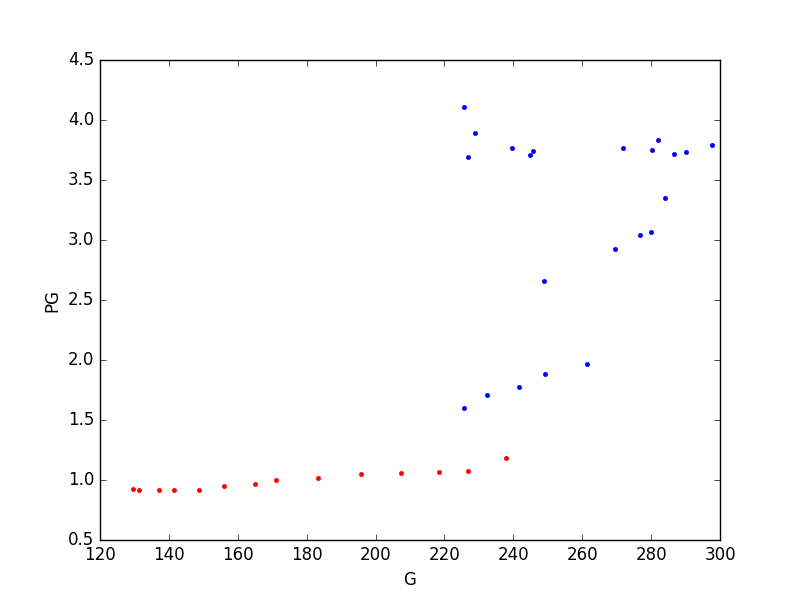
\includegraphics[height=6cm]{stat_tests2_02.png}

1973 ve 1980'deki fiyat zıplamaları net bir şekilde görülüyor, ayrıca
tüketimde de daha fazla değişkenlik / varyans mevcut. Eğer bu veriye bir
model uydurmak isteseydik, aynı modelin iki ayrı bölgeye her değişken için
aynı mükemmeliyette uymasını beklemek hayalcilik olurdu.

Test edeceğimiz model şöyle, 

\begin{minted}[fontsize=\footnotesize]{python}
model = 'Ln_G_Pop ~ Ln_Income_Pop + Ln_Pg + Ln_Pnc + Ln_Puc'
\end{minted}

Bu modeldeki fiyatlar \verb!G,Pnc,Puc!, sırasıyla benzin, yeni araba ve
kullanılmış araba fiyatları. \verb!Ln_G_Pop!, \verb!G! ile \verb!Pop!
(nüfus) bölünmesiyle elde ediliyor, ve \verb!Ln! notasyonumuz log işlemi
demek. \verb!Income! ülke geliri, o da \verb!Pop! ile bölünüyor ve log'u
alınıyor.

\begin{minted}[fontsize=\footnotesize]{python}
df['Ln_G_Pop'] = np.log(df.G/df.Pop)
df['Ln_Income_Pop'] = np.log(df.Y/df.Pop)
df['Ln_Pg'] = np.log(df.Pg)
df['Ln_Pnc'] = np.log(df.Pnc)
df['Ln_Puc'] = np.log(df.Puc)
\end{minted}

\begin{minted}[fontsize=\footnotesize]{python}
plt.plot(df.Year,df.Ln_G_Pop)
plt.xlabel('Sene')
plt.ylabel('Ln(G/Nufus)')
plt.title('Amerika Benzin Tuketimi')
plt.savefig('stat_tests2_03.png')
\end{minted}

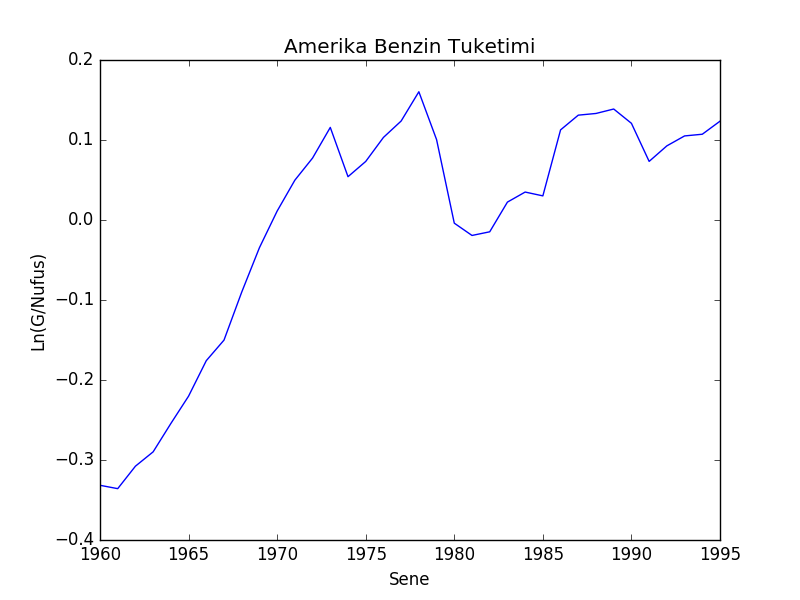
\includegraphics[height=6cm]{stat_tests2_03.png}

Modeli tüm veri üzerinde işletirsek,

\begin{minted}[fontsize=\footnotesize]{python}
import statsmodels.formula.api as smf
res_r = smf.ols(model, data=df).fit()
print res_r.summary()
\end{minted}

\begin{verbatim}
                            OLS Regression Results                            
==============================================================================
Dep. Variable:               Ln_G_Pop   R-squared:                       0.969
Model:                            OLS   Adj. R-squared:                  0.965
Method:                 Least Squares   F-statistic:                     243.2
Date:                Thu, 12 Jan 2017   Prob (F-statistic):           6.25e-23
Time:                        14:06:38   Log-Likelihood:                 79.913
No. Observations:                  36   AIC:                            -149.8
Df Residuals:                      31   BIC:                            -141.9
Df Model:                           4                                         
Covariance Type:            nonrobust                                         
=================================================================================
                    coef    std err          t      P>|t|      [95.0% Conf. Int.]
---------------------------------------------------------------------------------
Intercept        -7.7892      0.359    -21.679      0.000        -8.522    -7.056
Ln_Income_Pop     2.1175      0.099     21.443      0.000         1.916     2.319
Ln_Pg            -0.0979      0.028     -3.459      0.002        -0.156    -0.040
Ln_Pnc            0.1224      0.112      1.092      0.283        -0.106     0.351
Ln_Puc           -0.1022      0.069     -1.475      0.150        -0.243     0.039
==============================================================================
Omnibus:                        2.323   Durbin-Watson:                   0.891
Prob(Omnibus):                  0.313   Jarque-Bera (JB):                1.281
Skew:                           0.049   Prob(JB):                        0.527
Kurtosis:                       2.081   Cond. No.                         319.
==============================================================================

Warnings:
[1] Standard Errors assume that the covariance matrix of the errors is correctly specified.
\end{verbatim}

Şimdi her iki parça üzerinde ayrı ayrı regresyon işletelim, ki parçaları
1973 değeri üzerinden oluşturacağız, bu bildiğimiz bir değer ve bir anlamda
bu değerin gerçekten bir kopuş noktası olup olmadığını test etmek
istiyoruz, ve ardından Chow testi için gerekli değerleri hesaplıyoruz,

\begin{minted}[fontsize=\footnotesize]{python}
df_x = df[['Ln_Income_Pop','Ln_Pg','Ln_Pnc','Ln_Puc']]
df_y = df['Ln_G_Pop']

print len(df[df.Year<=1973]), len(df[df.Year>1973])
res1 = smf.ols(model, data=df[df.Year<1974]).fit()
res2 = smf.ols(model, data=df[df.Year>=1974]).fit()
S_1 = np.sum(res1.resid**2)
S_2 = np.sum(res2.resid**2)
S_r = np.sum(res_r.resid**2)
print 'S 1 =', S_1
print 'S 2 =', S_2
print 'S_r =', S_r
print 'N =', len(df)
k = df_x.shape[1]
tmp1 = (S_r-(S_1+S_2))/k
tmp2 = (S_1+S_2)/(len(df)-2*k-1)
F = tmp1/tmp2
print 'F =', F

import scipy.stats as st
f = st.f(k,len(df)-2*k-1)
print 'p degeri =', 1-f.cdf(F)
\end{minted}

\begin{verbatim}
14 22
S 1 = 0.00256733994753
S 2 = 0.00491175470666
S_r = 0.024873436262
N = 36
F = 15.6986655847
p degeri = 9.40286063456e-07
\end{verbatim}

Hesaplanan p değeri çok küçük, ve 0.05'ten daha az, demek ki hipotez
reddedildi. Demek ki hakikaten 1973'te bir değişim olmuş!

Değişim Noktasını Bulmak

Eğer değişim anı 1973'ü bilmeseydik onu nasıl ortaya çıkartırdık? Bir
yaklaşıma göre [5] tüm seneleri teker teker deneyerek Chow testini ardı
ardına işletebilirdik ve elde edilen en büyük F değeri bize değişim
noktasını verirdi. Bu kodu işletirsek,

\begin{minted}[fontsize=\footnotesize]{python}
import numpy as np
from numpy.linalg import pinv
def supf(y, x, p):
    N = y.shape[0]
    range = np.floor(np.array([N * p, N * (1 - p)]))
    range = np.arange(range[0], range[1] + 1, dtype=np.int32)
    x = x - np.mean(x)
    y = y - np.mean(y)
    e = smf.OLS(y,x).fit().resid
    S_r = np.sum(e**2)
    k = x.shape[1]
    print 'N =',N
    print 'k =',k
    print 'N-k =',N-k
    F_stat = np.zeros(N)
    for t in range:
        X1 = x[:t]
        X2 = x[t:]
        e[:t] = smf.OLS(y[:t],X1).fit().resid
        e[t:] = smf.OLS(y[t:],X2).fit().resid
        R2_u = 1 - e.dot(e) / y.dot(y)
        S_u = np.sum(e**2)
        F_stat[t] = ((S_r - S_u) / k) / (( S_u) / (N-2*k))
    return F_stat.argmax(),F_stat.max()
    
p = 0.2

idx,val = supf(df_y, df_x, p)
print idx,val
print 'Sene', df.Year[idx]
\end{minted}

\begin{verbatim}
N = 36
k = 4
N-k = 32
14 3.9049721931
Sene 1974
\end{verbatim}

Not: Sene araması için baştan ve sonda bir kısım veri atlandı, ki her iki
parça için elde yeterli veri olabilsin. 

Not: \verb!lmfit! hakkında bazı tavsiyeler için bkz [12] yazısı.

Sonucu 1974 olarak bulduk. Fena değil!


Kaynaklar

[1] Hill, {\em Principles of Econometrics}

[2] Uriel, {\em Introduction to Econometrics, Lecture}

[3] Haslwanter, {\em Introduction to Statistics Using Python}

[4] Wackerly, {\em Mathematical Statistics, 7th Edition}

[5] Soong, {\em Fundamentals of Probability and Statistics for Engineers}

[6] OCW MIT, {\em Statistics for Applications, 18.443}

[7] Hunter, {\em Asymptotics for Statisticians}

[8] Steiger, {\em Correlation and Regresion, Lecture Notes}

[9] Sheppard, {\em Introduction to Python for Econometrics}

[10] Greene, {\em Econometric Analysis}

[11] Uriel, {\em Introduction to Econometrics}

[12] Bayramli, Istatistik, {\em Gayri Lineer Regresyon, Petrol Tepe Noktası}

\end{document}
